\documentclass{article}
\usepackage[utf8]{inputenc}
\usepackage{physics}
\usepackage{amsmath}
\usepackage{showlabels}
\usepackage{amssymb}
\title{Statistical Computing for Scientists and Engineers\\[1em] Homework 5}
\author{Jiale Shi}
\date{Nov/12/2018}

\usepackage{natbib}
\usepackage{graphicx}
\usepackage{array}
\begin{document}
\maketitle

\newpage

\section{Importance Sampling}
Use importance sampling to approximate expectation $\mathbb{E}_{p}[f(x)]$ where
\begin{equation}
    f(x) = 2\sin(\frac{\pi}{1.5}x) , x\geq 0
\end{equation}
and target distribution is defined as 
\begin{equation}
    p(x) = x^{1.65-1}\exp(-x^2/2), x\geq 0
\end{equation}

write down your choice of sampling distribution. Plot sampling distribution and target distribution on a plot. Write down the algorithm of your implementation.

Solution:
The target distribution 
\begin{equation}
    p(x) = x^{1.65-1}\exp(-x^2/2) =x^{0.65}\exp(-x^2/2) , x\geq 0
\end{equation}

The shape of the target distribution is similar to the Gamma distribution Gamma(3,2.5) to some extent. Therefore, we choose Gamma distribution Gamma(3,2.5) as our proposed distribution.

\begin{figure}[h!]
\centering
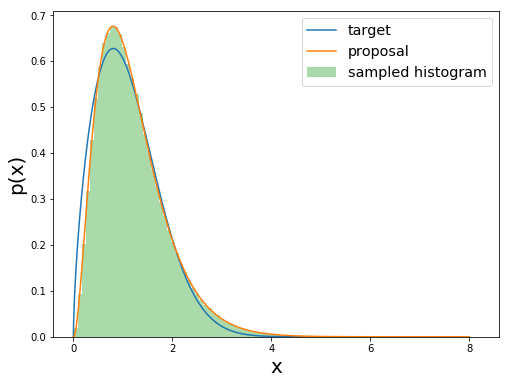
\includegraphics[scale=0.6]{HW5P1_1.png}
\caption{sampling distribution Gamma(3,2.5), target distribution}
%\label{fig:universe}
\end{figure}

We samples for $N = 10^6$ times, collect samples(x), calculate weight$W$.
\begin{equation}
    W(samples) = \frac{p(samples)}{Gamma(3,2.5)}
\end{equation}

\begin{equation}
    E(f(x)) \approx \frac{1}{N}\sum_{i=1}^{N}W(samples)f(samples) \approx 0.7758554717760647
\end{equation}



\newpage
\section{Sequential Monte Carlo Sampler}
Implement a sequential Monte Carlo sampler to draw samples from target distribution $\pi$, which is an equal mixture of 5 normal distributions in $\mathbb{R}^2$ with unit covariance and centers that are equally distributed on the circumference of a circle with diameter 40.

Initialize 3000 particles with points located at the center of the circle.

Using 100 bridging densities $\pi_{0}$,... ,$\pi_{100}$ where
\begin{equation}
    \pi_{k}(x) \propto \pi(x)^{\alpha_{k}}
\end{equation}
and $0 \leq \alpha_{1} \leq ... \leq \alpha_{n} = 1$.

Use a normal random walk proposal with step size $\sqrt{6}$ to evolve particles

Measure degeneracy using effective sample size with a threshold of $N/2$ and resample accordingly.

To show the evolution of the points, including distribution of points for $\pi_{0}$, $\pi_{50}$, $\pi_{100}$. Additionally, generate an animation showing the points evolving from $\pi_{0}$ to $\pi_{n}$. Write down algorithm of your implementation.

Solution:
Target distribution $\pi$, is an equal mixture of 5 normal distributions in $\mathbb{R}^2$ with unit covariance and centers that are equally distributed on the circumference of a circle with diameter 40.

The five center points should be

$(x_1,y_1) = (20\cos(0),20 \sin(0))$ ; 

$(x_2,y_2) = (20\cos(\frac{2\pi}{5}),20 \sin(\frac{2\pi}{5}))$; 

$(x_3,y_3) = (20\cos(\frac{4\pi}{5}),20 \sin(\frac{4\pi}{5}))$; 

$(x_4,y_4) = (20\cos(\frac{6\pi}{5}),20 \sin(\frac{6\pi}{5}))$; 

$(x_5,y_5) = (20\cos(\frac{8\pi}{5}),20 \sin(\frac{8\pi}{5}))$

The final target distribution $\pi(x,y)$ should  be
\begin{equation}
\begin{aligned}
    \pi(x,y) =   & \exp\{ -[(\frac{(x-x_1)^2}{2})+(\frac{(y-y_1)^2}{2})] \} \\
     + & \exp\{-[(\frac{(x-x_2)^2}{2})+(\frac{(y-y_2)^2}{2})] \} \\
     + & \exp\{-[(\frac{(x-x_3)^2}{2})+(\frac{(y-y_3)^2}{2})] \} \\
     + & \exp\{-[(\frac{(x-x_4)^2}{2})+(\frac{(y-y_4)^2}{2})] \}   \\
     + & \exp\{-[(\frac{(x-x_5)^2}{2})+(\frac{(y-y_5)^2}{2})] \}
\end{aligned}
\end{equation}

All the 3000 particles start from the original point $(0,0)$.
For $K = [1,2,3,...,100]$, $a_{K} = [0.01,0.02,0.03,..,1]$ the target distribution $\pi(x,y)_{K} = \pi(x,y)^{a_K}$. The proposal distribution is a 2D normal distribution with step size is $\sqrt{6}$. The update follows the MH algorithm. The detail is in the following figure.

\begin{figure}[h!]
\centering
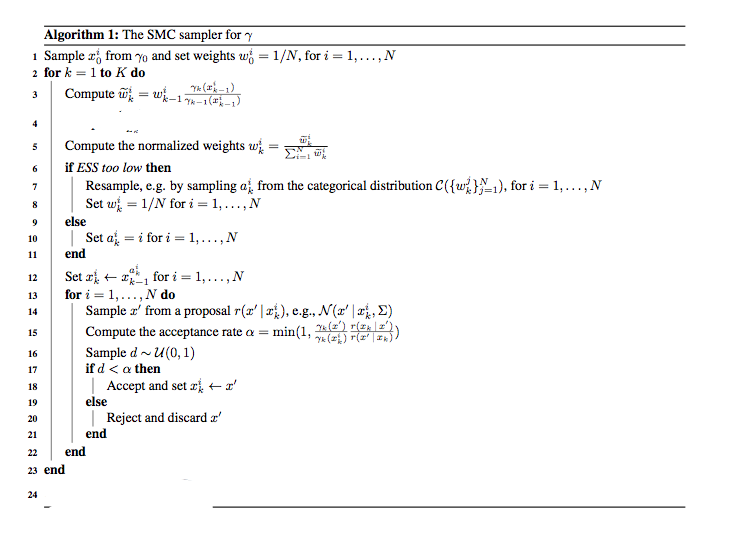
\includegraphics[scale=0.46]{SMCalgorithm.png}
\caption{SMC Algorithm}
%\label{fig:universe}
\end{figure}

The distribution of points for $\pi_{0}$, $\pi_{50}$,$\pi_{100}$.


\begin{figure}[h!]
\centering
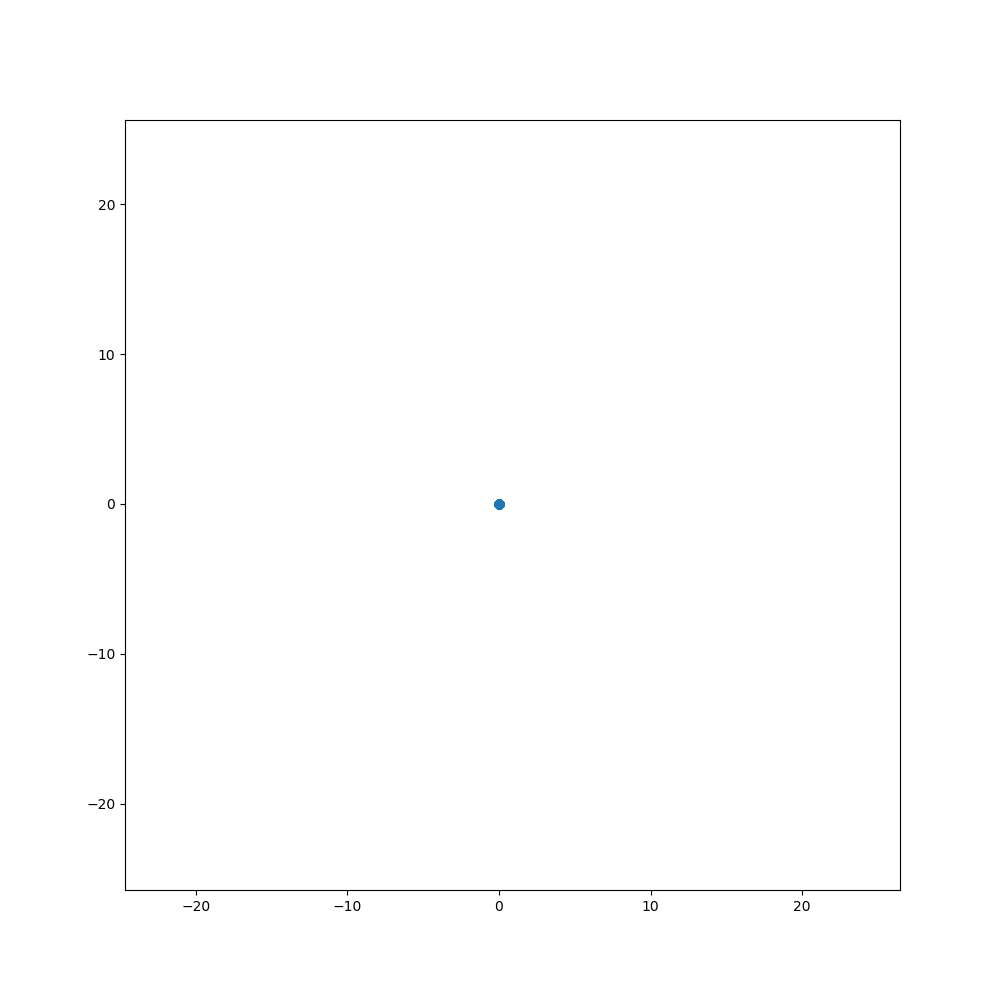
\includegraphics[scale=0.3]{f0.png}
\caption{$\pi_{0}$ start from the center of the circle}
%\label{fig:universe}
\end{figure}

\begin{figure}[h!]
\centering
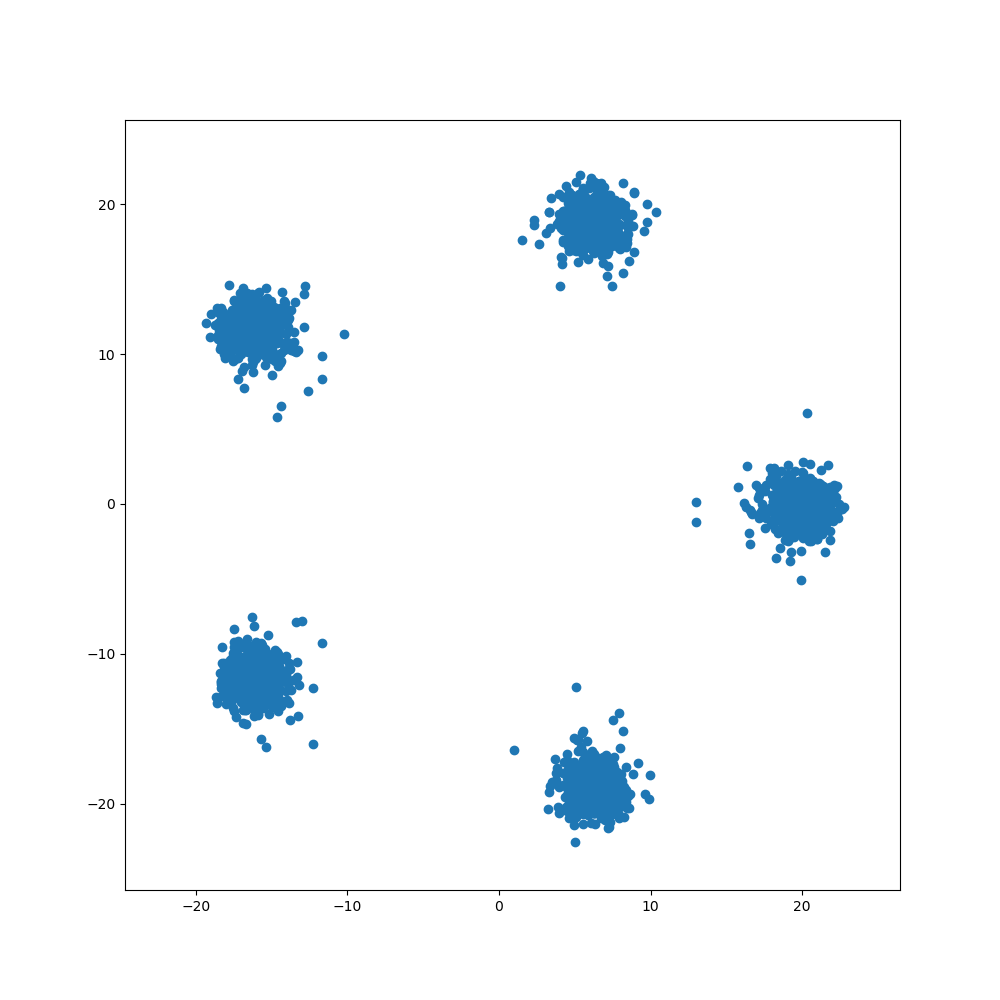
\includegraphics[scale=0.3]{f50.png}
\caption{$\pi_{50}$}
%\label{fig:universe}
\end{figure}

\begin{figure}[h!]
\centering
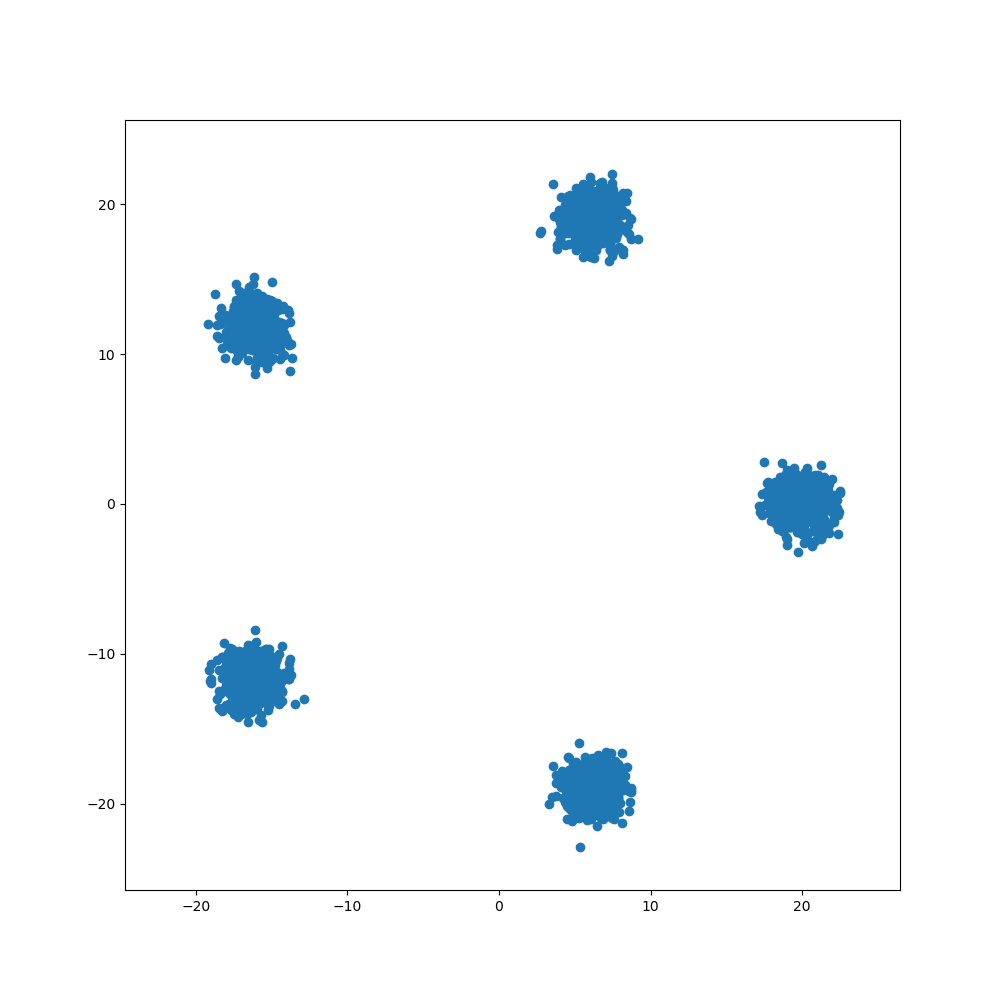
\includegraphics[scale=0.3]{f100.png}
\caption{$\pi_{100}$}
%\label{fig:universe}
\end{figure}




\newpage
\section{Hamiltonian Monte Carlo (HMC)}
HMC introduces an momentum variable $q$, and uses Hamiltonian dynamics to generate samples.


The potential energy $U(x) = -\log p(x)$, the kinetic energy $K(q) = -\log p(q)$.
$p(x)$ is the target density and $p(q)$ is the proposal density for $q$.
The summation $H(x,q) = U(x) + K(q)$. If we can generate samples $\propto \exp(-H(x,q)) = p(x)p(q)$, the resulting x samples will be distributed according to the target one.

To generate new candidate samples based on the Hamilton's equation of motion:

\begin{equation}
\begin{aligned}
& \frac{\partial x_i}{\partial t} = & \frac{\partial H}{\partial q_i} = & \frac{\partial K}{\partial q_{i}} \\
& \frac{\partial q_i}{\partial t} = & -\frac{\partial H}{\partial x_i} = & -\frac{\partial U}{\partial x_{i}}
\end{aligned}
\end{equation}

For numerical implementation, Hamilton's equations must be approximated by non-continual time, using small step $\epsilon$. 
It starts with half step update for the momentum variable, and then do a full step for $x$ using the update momentum, and then do the other half step for momentum.
\begin{equation}
\begin{aligned}
& q_{i}(t+\epsilon/2) = q_i(t) -(\epsilon/2)\frac{\partial U}{\partial x_{i}(t)} \\
& x_{i}(t+\epsilon) = x_{i}(t)+ \epsilon   \frac{\partial H}{\partial q_i}  & \mbox{where}  &  \frac{\partial H}{\partial q_i}=q_i(t+\epsilon/2) \\ %\frac{\partial K}{\partial q_{i}}
& q_{i}(t+\epsilon) = q_i(t+\epsilon/2) -(\epsilon/2)\frac{\partial U}{\partial x_{i}(t+\epsilon)} 
\end{aligned}
\end{equation}


\begin{figure}[h!]
\centering
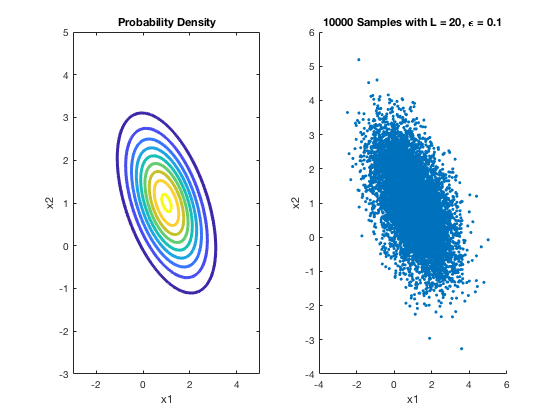
\includegraphics[scale=0.6]{HW5P3_1.png}
\caption{target distribution, sampled distribution}
%\label{fig:universe}
\end{figure}

\begin{figure}[h!]
\centering
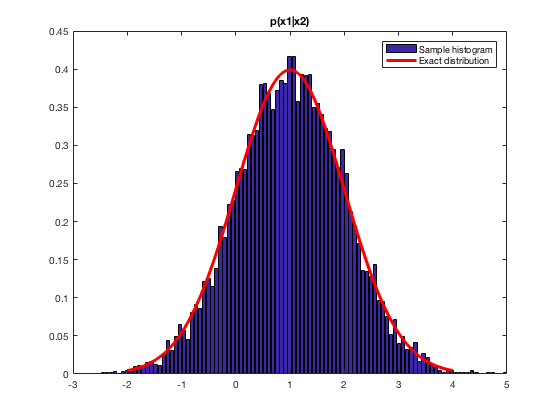
\includegraphics[scale=0.50]{HW5P3_2.png}
\caption{$p(x_1 | x_2)$}
%\label{fig:universe}
\end{figure}

\begin{figure}[h!]
\centering
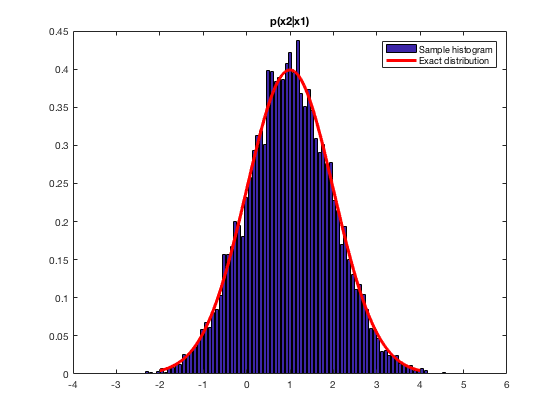
\includegraphics[scale=0.55]{HW5P3_3.png}
\caption{$p(x_2 | x_1)$}
%\label{fig:universe}
\end{figure}

\begin{figure}[h!]
\centering
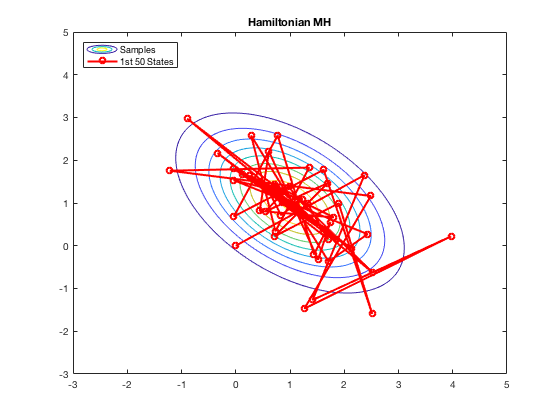
\includegraphics[scale=0.55]{HW5P3_4.png}
\caption{The first 50 steps}
%\label{fig:universe}
\end{figure}

\begin{figure}[h!]
\centering
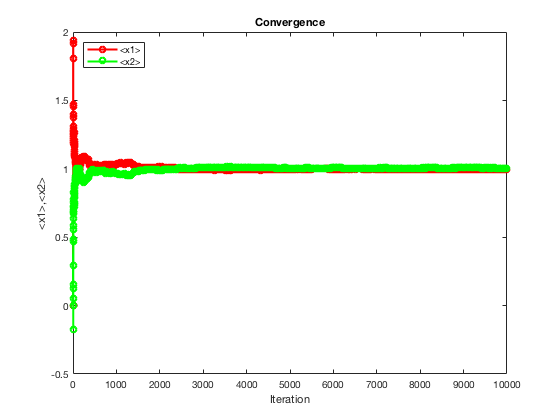
\includegraphics[scale=0.5]{HW5P3_5.png}
\caption{Convergence of $<x_{1}>, <x_{2}>$}
%\label{fig:universe}
\end{figure}




\newpage
\section{Sequential Importance Sampling for Solving Integral Equations}
Devise and implement a (sequential) importance sampling Monte Carlo scheme to solve the following integral equation for $f(x)$ (defined in [-1,1]) at $x=0$:

\begin{equation}
    f(x) = x+\frac{1}{2}\int^{1}_{-1}(t-x)f(t)dt
\end{equation}

and compare results with the actual solution:

\begin{equation}
    f(x) = \frac{3}{4}x+\frac{1}{4}
\end{equation}

Consider uniform distribution $U[-1-\alpha,1+\alpha]$ as the transition kernel and with the appropriate stopping rule (similarly to the example considered in class in solving $Ax=b$). Comment on the performance for $[\alpha=0.001,0.1,1,1.5,2]$

\textbf{Solution:}

According to the actual solution, $f(x) = \frac{3}{4}x+\frac{1}{4}$. 
The true value $f(0) = 0.25$. 

The integral equation can be transformed into solving
\begin{equation}
    f(x) = x + \sum_{n=1}^{\infty} \int_{-1}^{1} (\prod_{k=1}^{n}(t_{k}-t_{k-1}))t_k dt_{1:n}
\end{equation}
It involves an infinite sum of integrals of increasing dimension, which can be solved by SIS.
Consider uniform distribution $U[-1-\alpha,1+\alpha]$ as the transition kernel.

\begin{math}
\begin{aligned}
& P_{d} = \alpha \\
& M = \frac{1}{(2+2\cdot\alpha)} \\
\end{aligned}
\end{math}

simulate a path using Markov chain. Start from $x^{(i)}=0$, then generate sample $t_{1}^{(i)} \sim M(t_{1}^{(i)},t)$, $t_{2}^{(i)} \sim M(t_{2}^{(i)},t)$, until $t_{k+1}^{(i)}$ reaches $s$, the cemetery state.

Calculate the associated weight

\begin{math}
\begin{aligned}
W^{(i)} (x,t_{1},..,t_{k}) =     \left\{ \begin{array}{rcl}
     \frac{0.5((t_{1}-x))}{M} (\prod^{n}_{k=1} \frac{0.5(t_{k}-t_{k-1})}{M})\frac{t_{k}}{P_{d}} & \mbox{for}
   & k>0 \\ 
   \frac{0.5((t_{1}-x))}{M} \frac{t_{k}}{P_{d}} & \mbox{for} & k=0
 \end{array}\right.
\end{aligned}
\end{math}


\begin{math}
\begin{aligned}
f(x) = y^{(N)}  = \frac{y_{0} + \sum_{i}^{N}W^{(i)}}{N} & \mbox{where} & y_{0}=0
\end{aligned}
\end{math}

For $[\alpha=0.001,0.1,1,1.5,2]$, the performance is: 
\begin{equation}
\begin{aligned}
& \alpha = 0.001, & f(0) = 0.2764 & \mbox{slow}\\
& \alpha = 0.01, & f(0) = 0.2527 \\
& \alpha = 0.015, & f(0) = 0.2501 \\
& \alpha = 0.02, & f(0) = 0.2410 \\
& \alpha = 0.04, & f(0) = 0.2368 \\
& \alpha = 0.1, & f(0) = 0.2305 \\
& \alpha = 1, & f(0) = 0.1205 \\
& \alpha = 1.5, & f(0) = 0.0982 \\
& \alpha = 2, & f(0) = 0.0820 & \mbox{fast} 
\end{aligned}
\end{equation}

\begin{figure}[h!]
\centering
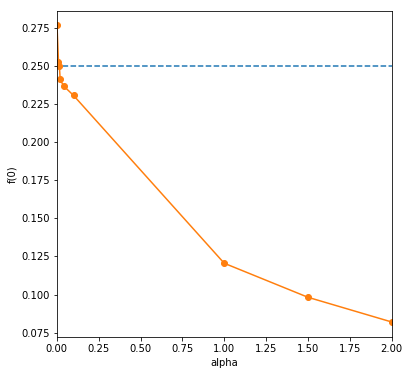
\includegraphics[scale=0.5]{HW5P4.png}
\caption{Convergence of $<x_{1}>, <x_{2}>$}
%\label{fig:universe}
\end{figure}

When $\alpha$ becomes larger and larger, the speed becomes faster and faster.
From $\alpha = [0.001,0.01,0.015,0.02, 0.04, 0.1,1,1.5,2]$, when $\alpha$ becomes larger and larger, $f(0)$ initially a little bigger than 0.25, and then $f(0)$ decreases. At $\alpha = 0.015$, $f(0)$ is closest to the true value 0.25.


%\bibliographystyle{plain}
%\bibliography{references}
\end{document}
